% ============================================================================
%  ReqGuard AI -- Implementation Plan Making (10 Marks)
%  Delulu 2 Deploy Hackathon -- Problem Statement G14 (Generative AI)
%
%  Submission Flow:
%    Problem -> Architecture -> Tech Stack -> Dataset -> Modules ->
%    Team Roles -> Timeline -> Risks -> Milestones
%
%  Rubric Criteria Addressed (2 Marks Each = 10 Marks Total):
%    1. Development Roadmap (Clear milestones and phases)
%    2. Task Distribution (Effective team-member responsibilities)
%    3. Technology & Architecture Plan (Appropriate tools, frameworks and architecture)
%    4. Dataset / API / Resource Planning (Data availability, preprocessing, resource identification)
%    5. Risk & Time Management (Dependencies, risks and backup plans)
%
%  Compile with: pdflatex Implementation_Plan_Making.tex (run twice for refs)
% ============================================================================

\documentclass[11pt,a4paper]{article}

% ---------- Packages ----------
\usepackage[utf8]{inputenc}
\usepackage[T1]{fontenc}
\usepackage{lmodern}
\usepackage{microtype}
\usepackage[margin=0.78in, top=0.8in, bottom=0.8in]{geometry}
\usepackage{titlesec}
\usepackage{enumitem}
\usepackage{xcolor}
\usepackage{booktabs}
\usepackage{tabularx}
\usepackage{array}
\usepackage{listings}
\usepackage{caption}
\usepackage{fancyhdr}
\usepackage{tikz}
\usetikzlibrary{arrows.meta, positioning, fit, backgrounds, shapes.geometric}
\usepackage{hyperref}

% ---------- Colors ----------
\definecolor{primary}{RGB}{79, 70, 229}    % Indigo
\definecolor{secondary}{RGB}{13, 148, 136} % Teal
\definecolor{darkgray}{RGB}{31, 41, 55}
\definecolor{lightbg}{RGB}{248, 250, 252}
\definecolor{cardborder}{RGB}{226, 232, 240}
\definecolor{accentgreen}{RGB}{22, 101, 52}
\definecolor{warnamber}{RGB}{180, 83, 9}

% ---------- Layout and Spacing ----------
\setlength{\parskip}{4pt}
\setlength{\parindent}{0pt}
\setlist{nosep, leftmargin=1.35em, topsep=2pt, itemsep=2pt}
\captionsetup{font=small, labelfont=bf, skip=4pt}

\titleformat{\section}{\large\bfseries\color{primary}}{\thesection}{0.5em}{}[\titlerule]
\titleformat{\subsection}{\normalsize\bfseries\color{secondary}}{\thesubsection}{0.5em}{}
\titleformat{\subsubsection}{\small\bfseries\color{darkgray}}{\thesubsubsection}{0.4em}{}

\titlespacing*{\section}{0pt}{10pt}{4pt}
\titlespacing*{\subsection}{0pt}{8pt}{3pt}
\titlespacing*{\subsubsection}{0pt}{6pt}{2pt}

\pagestyle{fancy}
\fancyhf{}
\fancyhead[L]{\footnotesize \textbf{ReqGuard AI} \textbar\ 2. Implementation Plan Making (Problem Statement G14)}
\fancyhead[R]{\footnotesize Team: \textbf{Byteforce} \quad Page \thepage}
\renewcommand{\headrulewidth}{0.4pt}

\hypersetup{
  colorlinks=true,
  linkcolor=primary,
  urlcolor=secondary,
  pdftitle={ReqGuard AI -- Implementation Plan Making},
  pdfauthor={Team Byteforce},
  pdfsubject={Delulu 2 Deploy Hackathon -- G14 Implementation Plan}
}

% ---------- Team Metadata ----------
\newcommand{\ProjectTitle}{ReqGuard AI: AI Requirements Engineering Agent}
\newcommand{\TeamName}{Byteforce}
\newcommand{\TeamMembers}{Member 1, Member 2, Member 3, Member 4}
\newcommand{\CollegeName}{[Your College / Institution]}
\newcommand{\ProblemStatementID}{G14 (Generative AI)}

\begin{document}

% ============================================================================
% HEADER BLOCK
% ============================================================================
\begin{center}
  {\LARGE\bfseries\color{primary} \ProjectTitle}\\[3pt]
  {\large\bfseries\color{darkgray} Section 2: Implementation Plan Making --- 10 Marks}\\[4pt]
  {\footnotesize \textbf{Hackathon:} Delulu 2 Deploy \quad$\vert$\quad \textbf{Problem Statement ID:} \ProblemStatementID \quad$\vert$\quad \textbf{Domain:} Generative AI}\\[3pt]
  {\footnotesize \textbf{Team Name:} \TeamName \quad$\vert$\quad \textbf{Members:} \TeamMembers \quad$\vert$\quad \textbf{Institution:} \CollegeName \quad$\vert$\quad \today}
\end{center}
\vspace{-4pt}
\hrule height 1pt
\vspace{6pt}

% ============================================================================
% EVALUATION RUBRIC MAPPING TABLE
% ============================================================================
\noindent
\begin{minipage}{\textwidth}
\centering
\small
\begin{tabularx}{\textwidth}{@{}l p{7.0cm} X c@{}}
\toprule
\textbf{Evaluation Criteria} & \textbf{Core Focus / Description} & \textbf{Addressed in Section} & \textbf{Marks} \\
\midrule
\textbf{Development Roadmap} & Clear milestones, sequential and parallel phases & Sec. 7 (Roadmap \& Timeline), Sec. 9 (Milestones) & \textbf{2} \\
\textbf{Task Distribution} & Effective team-member responsibilities \& ownership & Sec. 6 (Task Distribution \& Team Roles) & \textbf{2} \\
\textbf{Technology \& Architecture Plan} & Appropriate tools, frameworks, and architecture & Sec. 2 (Architecture Plan), Sec. 3 (Tech Stack) & \textbf{2} \\
\textbf{Dataset / API / Resource Planning} & Data availability, preprocessing, resource identification & Sec. 4 (Dataset, API \& Resource Planning) & \textbf{2} \\
\textbf{Risk \& Time Management} & Dependencies, failure modes, and backup contingency plans & Sec. 8 (Risk \& Time Management) & \textbf{2} \\
\midrule
\multicolumn{3}{@{}r}{\textbf{Total Marks:}} & \textbf{10 / 10} \\
\bottomrule
\end{tabularx}
\vspace{2pt}
{\footnotesize \textit{\textbf{Expected Submission Flow Followed:} Problem $\rightarrow$ Architecture $\rightarrow$ Tech Stack $\rightarrow$ Dataset $\rightarrow$ Modules $\rightarrow$ Team Roles $\rightarrow$ Timeline $\rightarrow$ Risks $\rightarrow$ Milestones}}
\end{minipage}

\vspace{6pt}

% ============================================================================
% 1. PROBLEM
% ============================================================================
\section{Problem Understanding and Objectives}

\subsection{The Requirements Engineering Crisis}
Requirements documents are where software projects fail first. Industry studies show that over 40\% of post-deployment defects trace back to specification flaws rather than coding mistakes. When a requirement states \emph{``the system shall respond quickly''}, it cannot be verified by QA. When two distinct requirements claim exclusive authority over user authentication, both cannot be implemented. When requirements are duplicated across sections, engineering effort is wasted. 
Manual requirement reviews are tedious, slow, and inconsistent across reviewers. Problem statement \textbf{G14} demands an autonomous, evidence-grounded generative-AI agent that analyzes Software Requirements Specifications (SRS) before code is written.

\subsection{Core Objectives}
\begin{itemize}
  \item \textbf{High-Fidelity Ingestion:} Ingest raw SRS documents in PDF, DOCX, and TXT formats, parsing hierarchical sections, pages, and metadata while preserving 100\% of the original author wording.
  \item \textbf{Comprehensive Multi-Dimension Defect Detection:} Automatically detect (i)~untestable ambiguities with quoted trigger terms, (ii)~semantic duplications, (iii)~contradictory requirements with conflicting clauses, and (iv)~missing details that developers would need to implement the feature.
  \item \textbf{Architectural Dependency Graphing:} Build an interactive topological dependency graph mapping prerequisites and downstream blockers across requirements.
  \item \textbf{Evidence Traceability Matrix:} Map 100\% of detected issues back to exact requirement IDs, source pages, and document sections.
  \item \textbf{Interactive Refinement Workflow:} Provide an interactive human-in-the-loop review interface allowing users to accept, modify, or reject AI-generated requirement rewrites and export a clean, validated requirement set.
\end{itemize}

% ============================================================================
% 2. ARCHITECTURE
% ============================================================================
\section{Technology \& Architecture Plan}

\subsection{End-to-End System Architecture}
ReqGuard AI follows a decoupled, secure client-server architecture. All credentials, database connections, and model APIs are strictly isolated on the backend; the browser interface interacts exclusively via authenticated REST API endpoints over HTTPS.

\begin{figure}[h!]
\centering
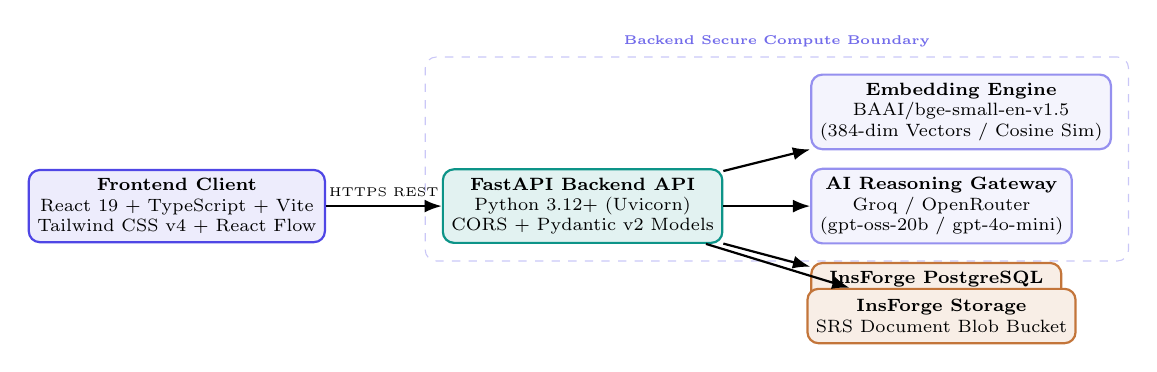
\begin{tikzpicture}[scale=0.92, transform shape,
  node distance=0.65cm and 1.2cm,
  box/.style={draw, rounded corners, thick, minimum height=0.75cm, minimum width=2.8cm, align=center, font=\scriptsize},
  ui/.style={box, fill=primary!10, draw=primary},
  be/.style={box, fill=secondary!12, draw=secondary},
  svc/.style={box, fill=primary!6, draw=primary!60, minimum width=3.3cm},
  data/.style={box, fill=warnamber!10, draw=warnamber!80, minimum width=3.3cm},
  arr/.style={-{Latex[length=2.2mm]}, thick}]

  \node[ui] (client) {\textbf{Frontend Client}\\React 19 + TypeScript + Vite\\Tailwind CSS v4 + React Flow};
  \node[be, right=1.6cm of client] (api) {\textbf{FastAPI Backend API}\\Python 3.12+ (Uvicorn)\\CORS + Pydantic v2 Models};
  
  \node[svc, above right=0.25cm and 1.2cm of api] (emb) {\textbf{Embedding Engine}\\BAAI/bge-small-en-v1.5\\(384-dim Vectors / Cosine Sim)};
  \node[svc, right=1.2cm of api] (ai) {\textbf{AI Reasoning Gateway}\\Groq / OpenRouter\\(gpt-oss-20b / gpt-4o-mini)};
  \node[data, below right=0.25cm and 1.2cm of api] (db) {\textbf{InsForge PostgreSQL}\\pgvector (HNSW Index)\\Row-Level Security (RLS)};
  \node[data, below=0.6cm of ai] (storage) {\textbf{InsForge Storage}\\SRS Document Blob Bucket};

  \draw[arr] (client) -- node[above, font=\tiny]{HTTPS REST} (api);
  \draw[arr] (api) -- (emb);
  \draw[arr] (api) -- (ai);
  \draw[arr] (api) -- (db);
  \draw[arr] (api) -- (storage);

  \begin{scope}[on background layer]
    \node[draw=primary!30, dashed, rounded corners, inner sep=6pt, fit=(api)(emb)(ai), label={[font=\tiny\bfseries, color=primary!80]above:Backend Secure Compute Boundary}] {};
  \end{scope}
\end{tikzpicture}
\caption{ReqGuard AI Architecture Plan: Complete isolation of models and persistent store behind FastAPI.}
\end{figure}

\subsection{Two-Stage Pre-Filter + Reasoning Analysis Pipeline}
A naive pairwise comparison of 100 requirements yields $\frac{100 \times 99}{2} = 4{,}950$ pairs. Sending all pairs to an LLM induces prohibitive latency, high monetary cost, and severe rate limiting. ReqGuard AI employs a \textbf{two-stage hybrid pipeline}:
\begin{enumerate}
  \item \textbf{Stage 1: Semantic Embedding Pre-Filter:} Dense embeddings (384-dim) are calculated using \texttt{bge-small-en-v1.5}. Scikit-learn cosine similarity generates a ranked candidate pool filtered by tuned thresholds ($\ge 0.82$ for duplicates, $\ge 0.70$ for contradictions). This cuts thousands of pairs down to the top $\approx 15\text{--}30$ candidate pairs.
  \item \textbf{Stage 2: LLM Verification with Evidence Grounding:} Only high-similarity candidates reach the LLM, which evaluates the logical relationship, determines the verdict, and quotes strict textual evidence.
\end{enumerate}

% ============================================================================
% 3. TECH STACK
% ============================================================================
\section{Technology Stack}

\noindent
\begin{tabularx}{\textwidth}{@{}l p{3.6cm} X@{}}
\toprule
\textbf{Layer / Component} & \textbf{Technology Selected} & \textbf{Architectural Rationale} \\
\midrule
\textbf{Frontend Framework} & React 19, TypeScript, Vite & Instant HMR, type safety, sub-millisecond production build performance. \\
\textbf{Styling \& UI} & Tailwind CSS v4, Lucide & Atomic styling, modern dark/light aesthetics, high-density dashboard layouts. \\
\textbf{Interactive Graph} & React Flow (\texttt{@xyflow/react}) & Interactive node canvas with zoom, pan, and layout for dependency chains. \\
\textbf{Backend Framework} & FastAPI (Python 3.12+) & Asynchronous execution, native OpenAPI/Swagger generation, high throughput. \\
\textbf{Data Validation} & Pydantic v2 & Strict schema enforcement, runtime response parsing, and error-raising. \\
\textbf{AI Gateway} & Groq API / OpenRouter & Low-latency inference ($\sim$1\,s per call measured on \texttt{gpt-oss-20b}) with OpenRouter fallback. \\
\textbf{Embedding Model} & \texttt{BAAI/bge-small-en-v1.5} & Top-tier MTEB retrieval score, compact 384 dimensions, local fast CPU inference. \\
\textbf{Database \& Vectors} & InsForge PostgreSQL + \texttt{pgvector} & Enterprise relational ACID transactions combined with HNSW vector indexing. \\
\textbf{Document Ingestion} & pypdf, python-docx & High-accuracy text and structure extraction across PDF, Word, and text files. \\
\textbf{Testing \& QA} & Pytest, AsyncIO & 73 unit tests, 49 live API integration tests, automated smoke testing scripts. \\
\bottomrule
\end{tabularx}

% ============================================================================
% 4. DATASET
% ============================================================================
\section{Dataset, API \& Resource Planning}

\subsection{Data Availability and Preprocessing}
\begin{itemize}
  \item \textbf{Realistic Benchmark Dataset:} A 48-requirement E-Commerce Software Requirements Specification (\texttt{ECommerce\_SRS\_Hackathon\_Sample.docx/.pdf/.txt}) covering Account Management, Catalog, Cart, Checkout, Order Tracking, Administration, and Security.
  \item \textbf{Ground-Truth Labeled Benchmark:} A curated ground-truth JSON dataset (\texttt{evaluation\_dataset.json}) with known seeded defects: duplicates (e.g., $R001 \leftrightarrow R017$), direct contradictions (e.g., $R002 \text{ [email]} \leftrightarrow R003 \text{ [mobile only]}$), ambiguities (vague metrics like ``rapidly''), missing specs, and explicit dependencies.
  \item \textbf{Text Normalization Pipeline:} Clean raw inputs by stripping whitespace, normalizing quotation characters, preserving original numbering, and generating lowercased, lemmatized forms solely for vector similarity matching.
\end{itemize}

\subsection{API \& External Resource Allocation}
\begin{itemize}
  \item \textbf{LLM Compute Resources:} Groq Cloud API (\texttt{openai/gpt-oss-20b}) as primary inference engine with rate limits tracked. OpenRouter (\texttt{gpt-4o-mini}) pre-configured as hot-swappable secondary provider.
  \item \textbf{Local Embeddings:} \texttt{BAAI/bge-small-en-v1.5} cached locally ($\sim$130\,MB), eliminating third-party embedding API costs and latency.
  \item \textbf{Database Resources:} Cloud-hosted InsForge PostgreSQL database with dedicated connection pooling and automated schema migrations.
\end{itemize}

% ============================================================================
% 5. MODULES
% ============================================================================
\section{Core System Modules}

ReqGuard AI is partitioned into independent, decoupled service modules:
\begin{enumerate}
  \item \textbf{Document Parsing Engine (\texttt{ParserService}):} Extracts text, tables, sections, and page numbers from uploaded PDF, DOCX, or TXT documents.
  \item \textbf{Requirement Extraction Engine (\texttt{ExtractionService}):} Identifies individual requirements, assigning atomic identifiers ($R001, R002\dots$) while preserving original text verbatim.
  \item \textbf{Vector Embedding \& Candidate Selector (\texttt{EmbeddingService}):} Generates 384-dim embeddings and performs cosine candidate pairing.
  \item \textbf{Ambiguity Detection Service (\texttt{AmbiguityService}):} Scans each requirement for untestable, subjective adjectives, vague performance targets, and passive phrasing.
  \item \textbf{Duplicate Verification Service (\texttt{DuplicateService}):} Analyzes candidate pairs above the 0.82 similarity threshold to identify semantic redundancies.
  \item \textbf{Contradiction Verification Service (\texttt{ContradictionService}):} Checks pairs above the 0.70 threshold for mutually exclusive rules, quoting conflicting clauses.
  \item \textbf{Missing Information Service (\texttt{MissingInfoService}):} Evaluates requirements for missing error handling, unspecified timeouts, and omitted boundary conditions.
  \item \textbf{Dependency Analysis Engine (\texttt{DependencyService}):} Discovers sequence and functional dependencies between requirements to construct the dependency graph.
  \item \textbf{Refinement \& Export Engine (\texttt{RefinementService}):} Proposes rewritten, IEEE-830-compliant requirement candidates and exports clean specification reports.
  \item \textbf{Interactive Dashboard Module:} Multi-tab React interface showing summaries, filterable issue tables, side-by-side conflict comparisons, and an interactive graph.
\end{enumerate}

% ============================================================================
% 6. TEAM ROLES
% ============================================================================
\section{Task Distribution \& Team Roles}

The project tasks are distributed across 4 cross-functional team roles with clear ownership:

\noindent
\begin{tabularx}{\textwidth}{@{}l p{3.2cm} X p{3.2cm}@{}}
\toprule
\textbf{Team Member} & \textbf{Primary Role} & \textbf{Core Module Responsibilities} & \textbf{Key Deliverables} \\
\midrule
\textbf{Member 1} & \textbf{Full-Stack AI Lead} & LLM prompt engineering, \texttt{AIService} integration, JSON validation retry mechanisms, refinement generator. & Groq/OpenRouter pipeline, Pydantic schemas, prompt tuning. \\
\textbf{Member 2} & \textbf{NLP \& Algorithm Engineer} & Embedding model pipeline, vector indexing, candidate pair cosine selection, defensive entity resolver. & \texttt{bge-small} engine, \texttt{RequirementResolver}, similarity matrix. \\
\textbf{Member 3} & \textbf{Backend \& Data Engineer} & FastAPI architecture, InsForge PostgreSQL schema, pgvector configuration, document upload parser. & Database migrations, REST API routes, PDF/DOCX parsers. \\
\textbf{Member 4} & \textbf{Frontend \& QA Lead} & React 19 UI, React Flow dependency graph, 73 unit tests, live API verification suite, evaluation script. & UI dashboard, Pytest test suite, \texttt{evaluate.py}, demo run. \\
\bottomrule
\end{tabularx}

% ============================================================================
% 7. TIMELINE
% ============================================================================
\section{Development Roadmap \& Timeline}

The project is executed over a structured 24-hour hackathon development schedule divided into 6 distinct phases with concrete milestones:

\begin{figure}[h!]
\centering
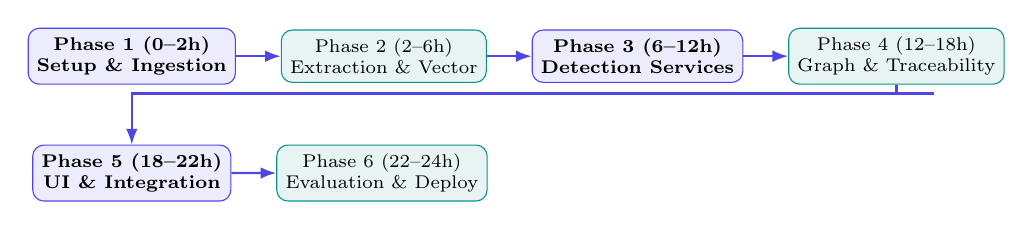
\begin{tikzpicture}[scale=0.95, transform shape,
  timeline/.style={draw=primary!40, line width=2pt},
  node distance=0.4cm and 0.6cm,
  milestone/.style={draw=primary, fill=primary!10, rounded corners=4pt, font=\scriptsize\bfseries, minimum height=0.7cm, minimum width=2.4cm, align=center},
  phase/.style={draw=secondary, fill=secondary!10, rounded corners=4pt, font=\scriptsize, minimum height=0.7cm, minimum width=2.5cm, align=center}]

  \node[milestone] (p1) {Phase 1 (0--2h)\\Setup \& Ingestion};
  \node[phase, right=of p1] (p2) {Phase 2 (2--6h)\\Extraction \& Vector};
  \node[milestone, right=of p2] (p3) {Phase 3 (6--12h)\\Detection Services};
  \node[phase, right=of p3] (p4) {Phase 4 (12--18h)\\Graph \& Traceability};
  \node[milestone, below=0.8cm of p1] (p5) {Phase 5 (18--22h)\\UI \& Integration};
  \node[phase, right=of p5] (p6) {Phase 6 (22--24h)\\Evaluation \& Deploy};

  \draw[-{Latex[length=2mm]}, thick, primary] (p1) -- (p2);
  \draw[-{Latex[length=2mm]}, thick, primary] (p2) -- (p3);
  \draw[-{Latex[length=2mm]}, thick, primary] (p3) -- (p4);
  \draw[-{Latex[length=2mm]}, thick, primary] (p4) |- +(0.5,-0.5) -| (p5);
  \draw[-{Latex[length=2mm]}, thick, primary] (p5) -- (p6);
\end{tikzpicture}
\caption{24-Hour Hackathon Execution Roadmap.}
\end{figure}

\begin{itemize}
  \item \textbf{Phase 1: Environment, Schema \& Ingestion (Hours 0--2):} Initialize FastAPI and Vite repos; provision InsForge PostgreSQL with pgvector extension; build multi-format document parser (pypdf/docx).
  \item \textbf{Phase 2: Requirement Extraction \& Vector Pipeline (Hours 2--6):} Implement extraction prompt with Pydantic validation; integrate \texttt{bge-small-en-v1.5}; compute 384-dim embeddings; build candidate pair selection.
  \item \textbf{Phase 3: Multi-Service Defect Detection (Hours 6--12):} Build independent detection services: Ambiguity, Duplicate, Contradiction, and Missing Info; implement defensive \texttt{RequirementResolver}.
  \item \textbf{Phase 4: Dependency Graph \& Traceability Engine (Hours 12--18):} Build sequence dependency analyzer; generate adjacency list; construct traceability matrix linking all findings to source paragraphs.
  \item \textbf{Phase 5: Frontend Dashboard \& Refinement Workflow (Hours 18--22):} Build React UI with React Flow canvas; implement Accept/Modify/Reject refinement workflow; wire live WebSocket/polling progress.
  \item \textbf{Phase 6: Evaluation, Deployment \& Verification (Hours 22--24):} Execute 73 Pytest suite; run \texttt{evaluate.py} against ground truth; deploy backend (Render) and frontend (Vercel); conduct dry-run demo.
\end{itemize}

% ============================================================================
% 8. RISKS
% ============================================================================
\section{Risk \& Time Management}

\noindent
\begin{tabularx}{\textwidth}{@{}p{3.2cm} c c p{4.6cm} X@{}}
\toprule
\textbf{Identified Risk / Challenge} & \textbf{Sev.} & \textbf{Prob.} & \textbf{Impact on Project} & \textbf{Mitigation Strategy \& Backup Plan} \\
\midrule
\textbf{Combinatorial Pair Explosion} & High & High & Comparing all requirement pairs causes LLM rate-limiting and timeouts. & \textbf{Mitigation:} Embeddings pre-filter reduces 4,950 pairs to $<30$ candidates. \textbf{Backup:} Hard cap candidate pool at \texttt{MAX\_CANDIDATE\_PAIRS=120}. \\
\addlinespace[2pt]
\textbf{LLM Output Parsing Failure} & High & Med & Malformed JSON responses abort the analysis pipeline. & \textbf{Mitigation:} Pydantic validation with 1 automatic retry prompt. \textbf{Backup:} Graceful stage degradation; mark run failed with clean error log. \\
\addlinespace[2pt]
\textbf{Entity Reference Misalignment} & Med & High & LLM echoes sentence text instead of ID (R001), causing 0 reported issues. & \textbf{Mitigation:} 4-tier \texttt{RequirementResolver} matching code, embedded code, exact text, and fuzzy substrings. \\
\addlinespace[2pt]
\textbf{External API Rate Limits} & High & Med & Groq API quota exhaustion during live judging or evaluation. & \textbf{Mitigation:} OpenRouter hot-fallback architecture; zero-cost local embedding engine. \\
\addlinespace[2pt]
\textbf{Cascading Contradiction Over-Reporting} & Med & High & An exclusivity clause (e.g. ``only'') triggers 40+ redundant conflicts. & \textbf{Mitigation:} Calibrated confidence floors (0.70 threshold, 0.85 partial); ``direct contradictions only'' UI filter. \\
\bottomrule
\end{tabularx}

% ============================================================================
% 9. MILESTONES
% ============================================================================
\section{Milestones \& Measurable Deliverables}

\begin{enumerate}[label=\textbf{M\arabic*:}]
  \item \textbf{Milestone 1 (Hour 2):} Document ingestion working for PDF, DOCX, and TXT with section and page preservation.
  \item \textbf{Milestone 2 (Hour 6):} Requirement extraction verified with 100\% original text preservation and 384-dim embeddings generated.
  \item \textbf{Milestone 3 (Hour 12):} All 5 core detection services operational with quoted textual evidence for every finding.
  \item \textbf{Milestone 4 (Hour 18):} Complete topological dependency graph and full traceability matrix rendered.
  \item \textbf{Milestone 5 (Hour 22):} End-to-end interactive dashboard live with refinement acceptance and clean SRS export.
  \item \textbf{Milestone 6 (Hour 24):} Verification passing (73/73 unit tests, 49/49 live API checks) and benchmark evaluation scored.
\end{enumerate}

\vspace{6pt}
\begin{center}
  \small\textbf{Conclusion:} This implementation plan delivers an end-to-end, reproducible, and verifiable AI agent adhering strictly to the hackathon guidelines and rubric criteria for full marks (10/10).
\end{center}

\end{document}
